\chapter{Ejecución del proyecto}
\label{chap:edp}
Este capítulo tiene como objetivo tratar el desarrollo del proyecto en si mismo, así como discutir las opciones disponibles durante el progreso y las decisiones tomadas para llevarlo a cabo.
\section{Consideraciones previas}
Este trabajo nace como un desarrollo del proyecto troncal de \citeauthor{IglesiasGuitian2022} y como tal se debe ceñir a las condiciones que acarrea dicho proyecto.
Todo el equipo utilizado durante el desarrollo fue provisto por parte del mismo, o en su defecto por parte del \acrfull{citic}.
\section{Dificultades}
Dada la naturaleza del trabajo (altamente dependiente del hardware para su ejecución), es necesaria la presencialidad a lo largo de gran parte del desarrollo. Por causa mayor me he visto obligado a desplazarme al otro extremo de la península, lo que ha condicionado en parte el final del proyecto.
\section{Estudio inicial}
Se llevó a cabo un estudio para definir la hoja de ruta del proyecto. Dada la problemática a solventar, este trabajo alcanza a tocar áreas bien diferenciadas entre si que se pueden destacar como los pasos a seguir del mismo:
\begin{itemize}
    \item Extracción de volúmenes 3D a partir de un \acrshort{tc} válidos para su impresión.
    \item Diseñar un marcador fiduciario que permita el seguimiento de una pieza en 3 dimensiones y un método de acople al volumen previamente impreso.
    \item Implementar una solución que permita el seguimiento de dicho marcador.
    \item Integrar la solución sobre un \acrshort{hmd}.
\end{itemize}

Fruto de la investigación surge el artículo de  \citeauthor{MoretaMartinez2020} que expone una solución existente a los objetivos de este trabajo mediante el uso de software bajo licencia o de pago.  Es por ello que se toma una aproximación similar al problema sobre todo en las fases iniciales para la generación de los volúmenes, a pesar de afrontar de forma distintas las casuísticas finales.
\section{Generación de volúmenes a partir de TC}
Con el fin de facilitar la validación del progreso del proyecto, se utilizo una \acrshort{tc} de pruebas. Dichos datos contienen la sección superior (hombros y cabeza) de un sujeto \ref{fig:manix_full}. Durante el desarrollo se sugirió como posible caso práctico seleccionar el cráneo del sujeto en los datos de prueba y trabajar en la alineación 3D sobre el mismo, por lo que en las siguientes figuras se representa este objetivo.

\begin{figure}[hp!]
  \centering
  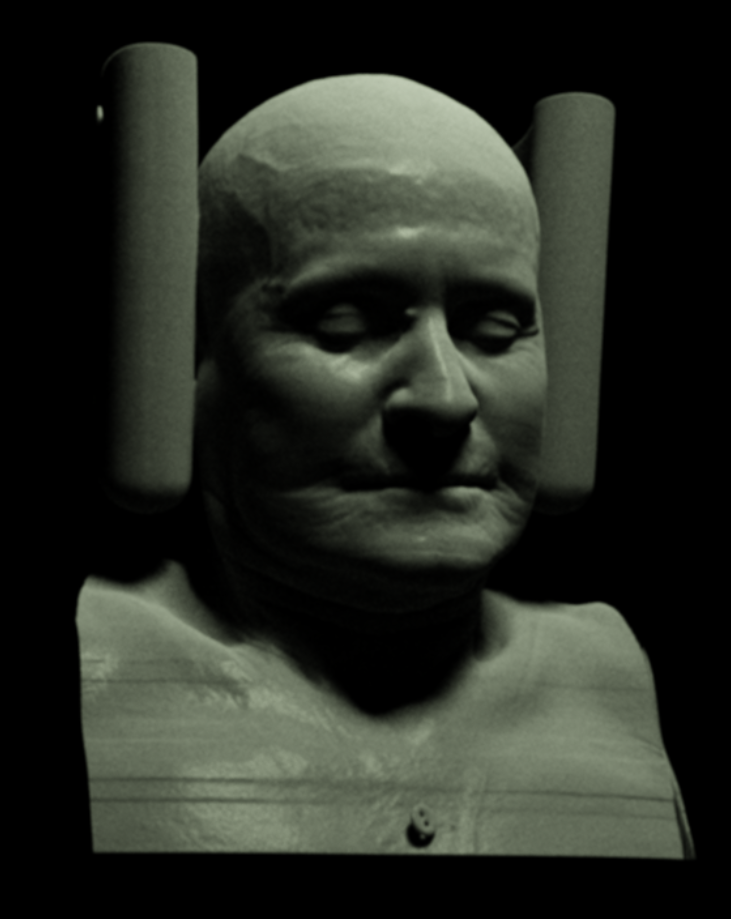
\includegraphics[width=0.75\textwidth]{imaxes/manix_full.png}
  \caption{Datos de prueba.}
  \label{fig:manix_full}
\end{figure}
Con el fin de seleccionar una sección concreta para exportar, se utilizaron las herramientas para segmentar volúmenes de Slicer3D
Nada mas abrir el programa se pueden ver las vistas, en las que se representará el \acrshort{tc} una vez se cargue \ref{fig:3dslier}.
Se utilizo principalmente la herramienta de "Thresholding" que permite seleccionar partes del modelo cuyas intensidades se comprenden en un intervalo o "threshold"  \ref{fig:seg_cr}. Posteriormente para eliminar las partes del modelo no deseadas se utilizo la herramienta de borrado hasta alcanzar el volumen deseado.

\begin{figure}%
    \centering
    \subfloat[\centering Captura de pantalla de 3DSlicer antes de cargar los datos.]{{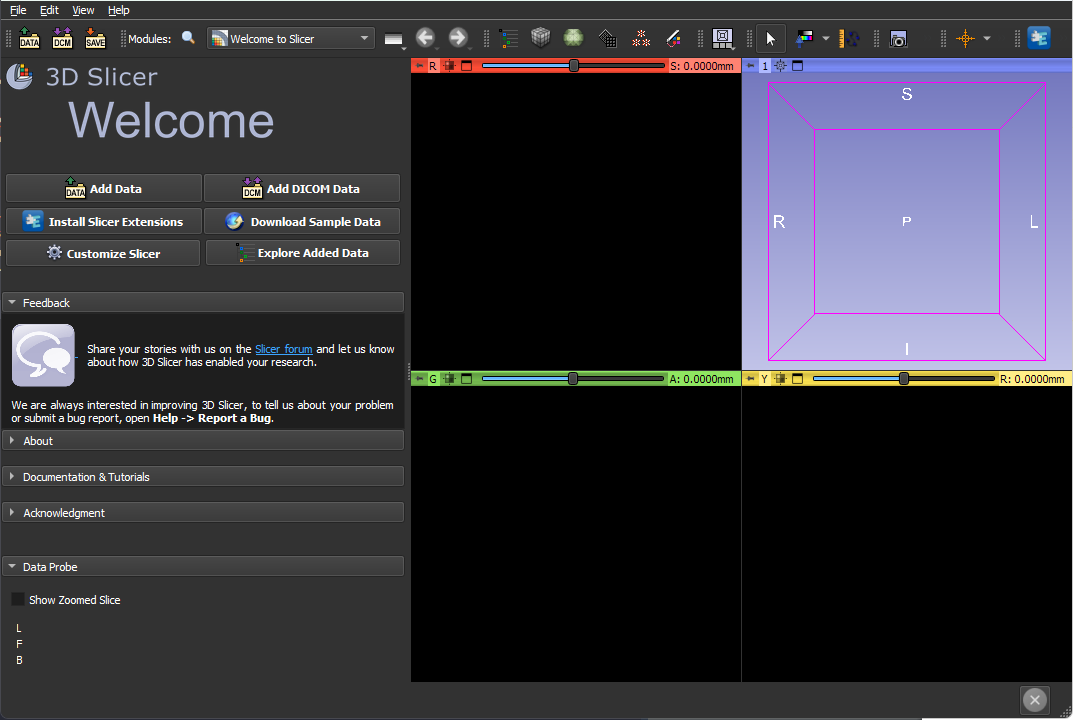
\includegraphics[width=6cm]{imaxes/captura3dslicer_1.png} }}%
    \qquad
    \subfloat[\centering  Captura de pantalla de 3DSlicer con los datos cargados.]{{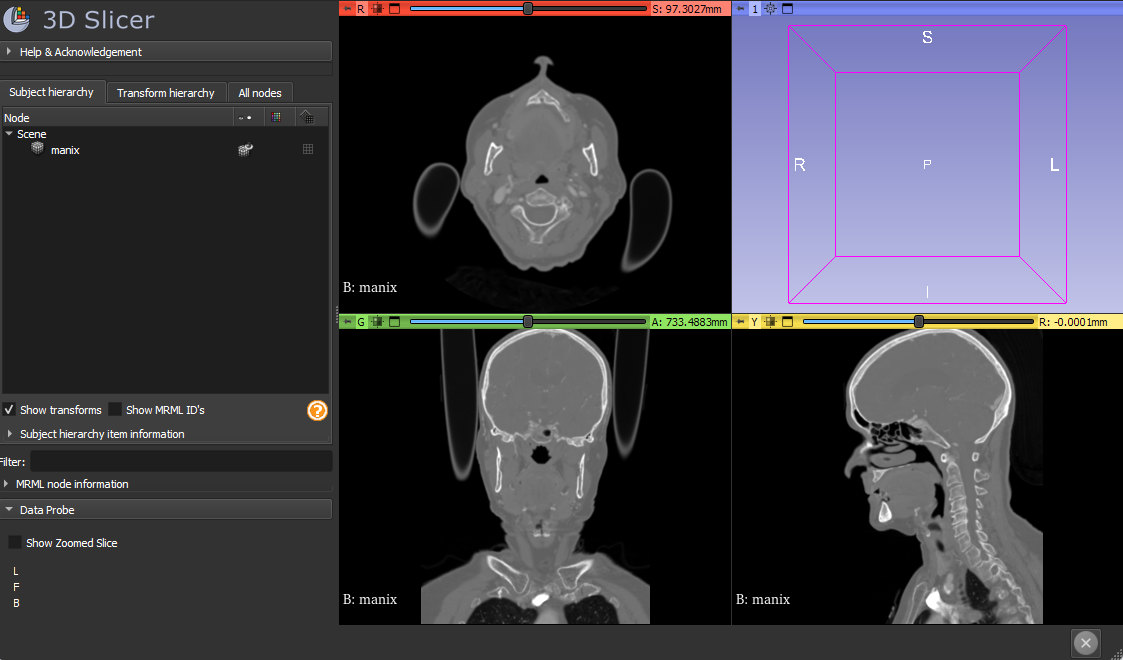
\includegraphics[width=6cm]{imaxes/captura3dslicer_2.png} }}%
    \caption{Capturas de 3DSlicer}%
    \label{fig:3dslier}%
\end{figure}


\begin{figure}[hp!]
  \centering
  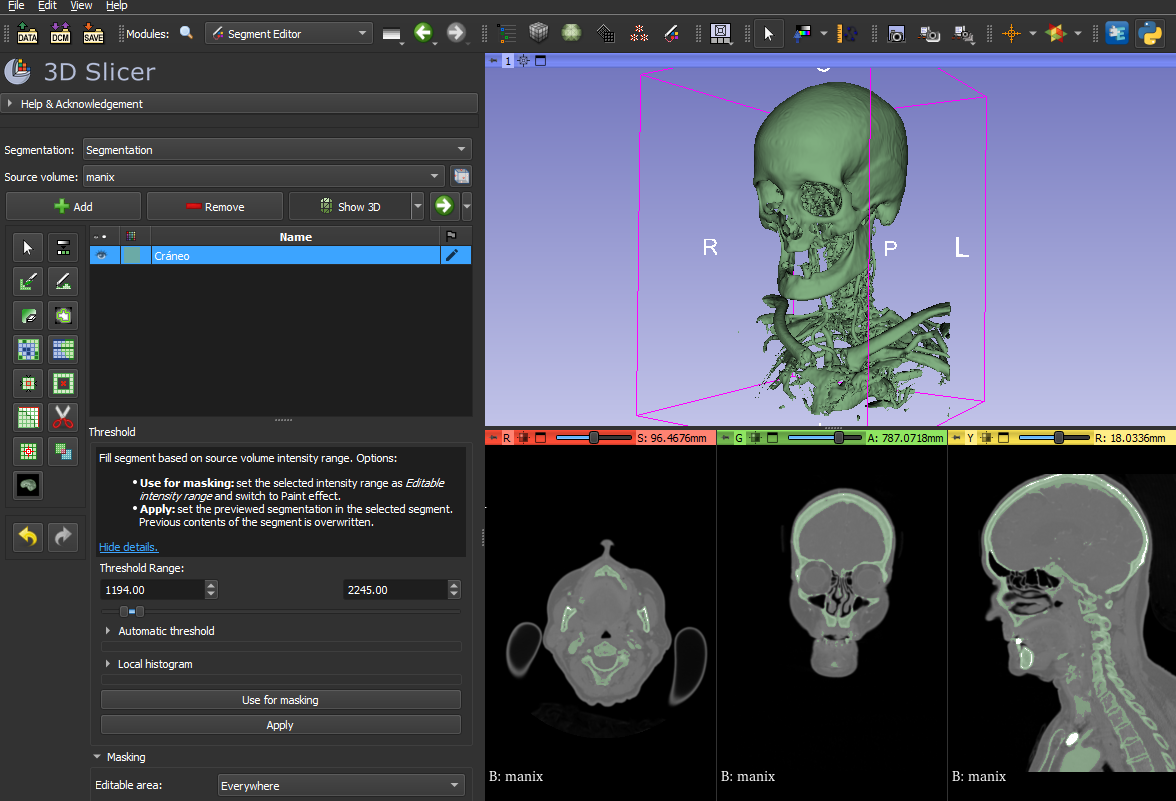
\includegraphics[width=0.75\textwidth]{imaxes/segment_craneo.png}
  \caption{Torso una vez aplicado el thresholding.}
  \label{fig:seg_cr}
\end{figure}
\section{Impresión 3D del volumen}
 Dado que el modelo no se genera a partir de figuras geométricas previas, es posible que presente geometrías rotas que a la hora del Slicing provocarán errores y no permitirán que se genere el GCODE correctamente.
 Por ello es necesario importar el modelo en un programa que nos facilite arreglar estas geometrías como es Meshmixer. En \ref{fig:arr_geo} se aprecia el modelo exportado, y cada marcador corresponde a errores producto de la exportación. Una vez reparados, se procede a imprimir la pieza.
 Como se comenta en \ref{chap:hs} para una pieza con una geometría tan compleja se requeriría una gran cantidad de soportes, por lo que se optó por la impresora Fuse 1 para la impresión de este modelo. A diferencia de una impresora 3D al uso, esta impresora utiliza un láser para fijar capa a capa el polvo de nylon, lo que garantiza una gran resolución en la pieza final y una gran durabilidad de la misma. Posterior al  trabajo de impresión es necesario retirar el material sobrante en la cámara de recuperación que cuenta con distintos utensilios para evitar malgastar el material sobrante ya que puede ser reutilizado.

\begin{figure}%
    \centering
    \subfloat[\centering Pieza en el proceso de recuperación del material.]{{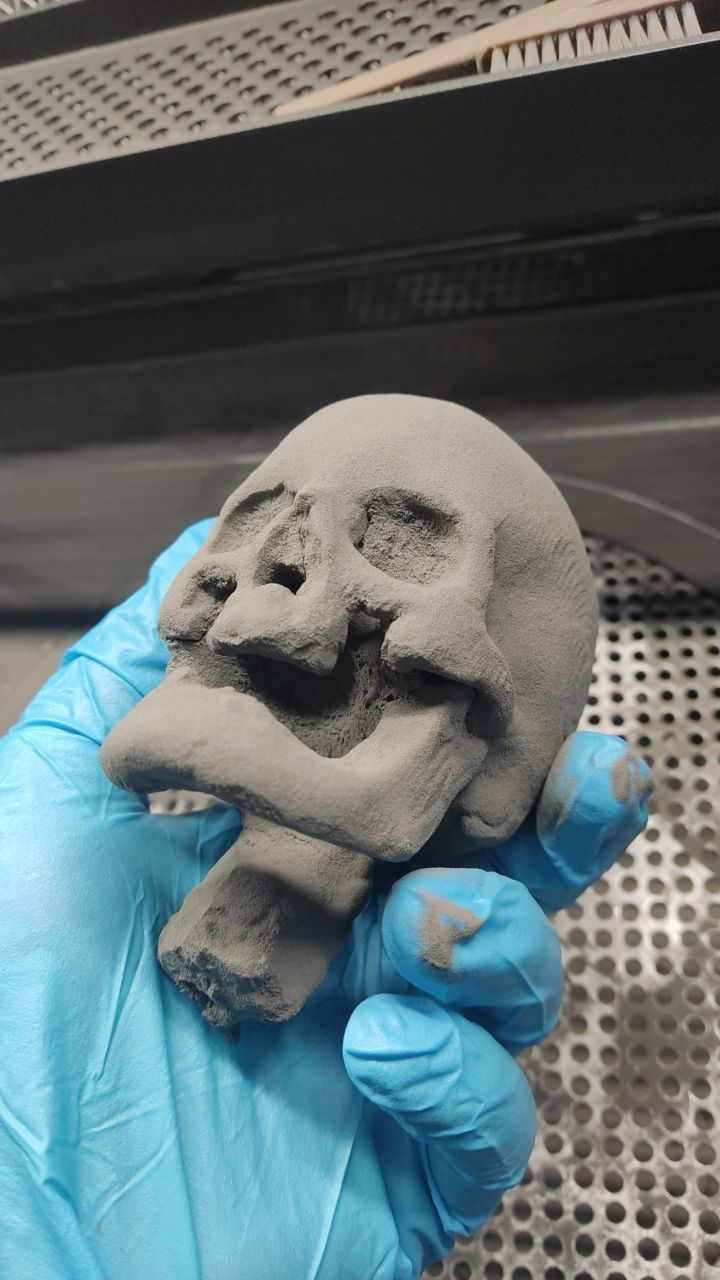
\includegraphics[width=6cm]{imaxes/limpiando_fig.png} }}%
    \qquad
    \subfloat[\centering  Pieza final.]{{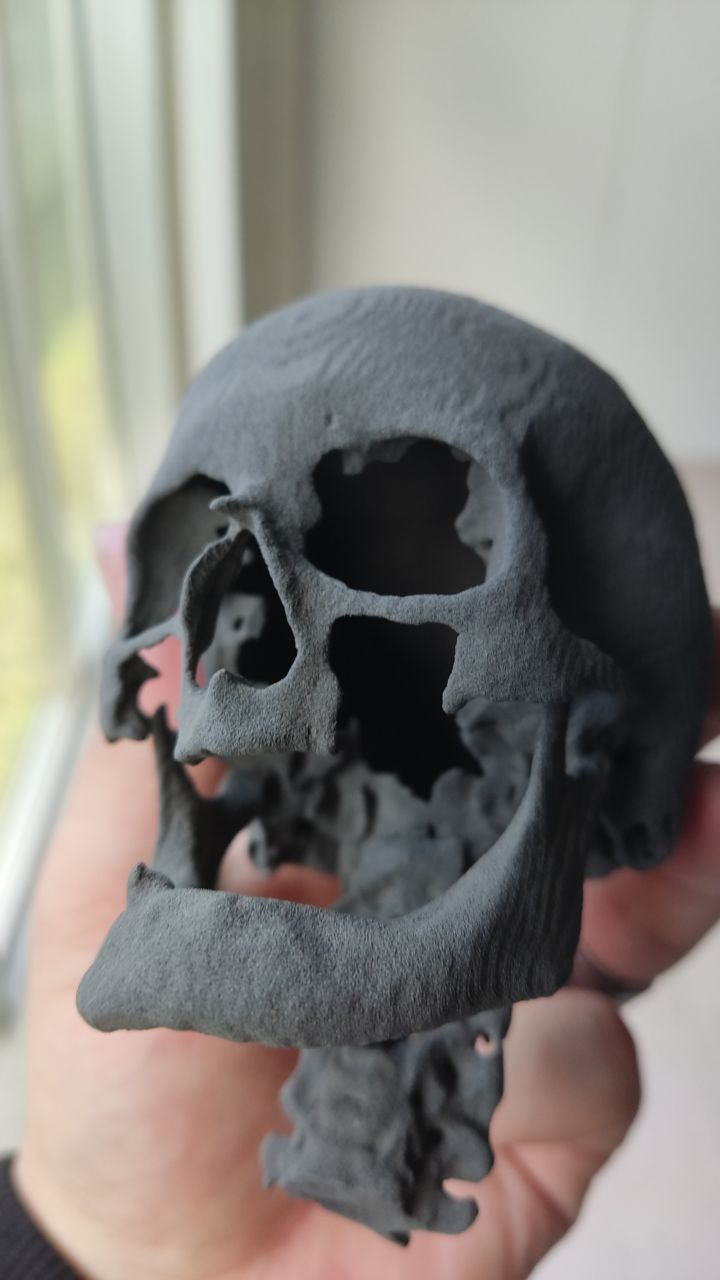
\includegraphics[width=6cm]{imaxes/limpia_fig.png} }}%
    \caption{Proceso de recuperación de material.}%
    \label{fig:3dslier}%
\end{figure}


\begin{figure}[hp!]
  \centering
  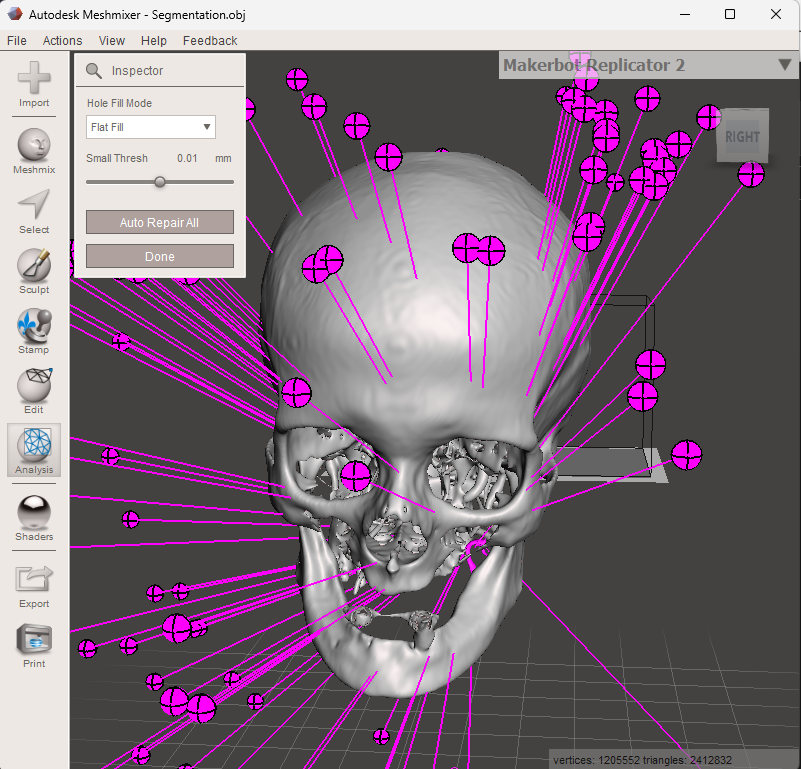
\includegraphics[width=0.75\textwidth]{imaxes/arreglo_geo.png}
  \caption{Modelo de cráneo 3D con geometrías erróneas.}
  \label{fig:arr_geo}
\end{figure}
 
\section{Desarrollo del marcador fiduciario}
Obtener la posición y rotación de una figura desconocida en el espacio es uno de los problemas principales a la hora de implementar soluciones de realidad virtual o aumentada, ya que requiere encontrar correspondencias entre objetos conocidos en el espacio y sus proyecciones en el vídeo.
Si bien existen aproximaciones que buscan puntos claves de las figuras o reconocen sus geometrías mediante técnicas de visión artificial e inteligencia artificial, se optó por el uso de  marcadores fiduciarios por varios motivos.
Primeramente, permite replicar el seguimiento del objeto independientemente del hardware utilizado, ya que una vez calibrada la cámara no se requiere ningún otro tipo de ajuste en el sistema. Otra ventaja es la robustez del sistema, ya que permite mantener el seguimiento a pesar de que parte del marcador se encuentre ocluido o no esté en el campo de visión de la cámara.
Dados los recursos disponibles, se optó por utilizar la librería ARuco para generar y seguir el marcador.
Debido a la versatilidad de las piezas con las que se pretende usar el marcador, se implementó priorizando eliminar las oclusiones del marcador por la pieza, por este motivo se diseñó como un cubo, de forma que al menos una cara sería visible en todo momento. A pesar de esto, utilizando un único marcador por cara cabe la posibilidad de que si parte del mismo se tapa, se pierda el seguimiento por completo dependiendo de que parte sea la afectada. Es por esto que se decidió implementar cada cara como una tabla de marcadores. Independientemente de la cara detectada el seguimiento se implementó de forma que se obtenga la rotación y posición del centro del cubo, transformando los valores obtenidos de cada cara para obtener este punto.

\paragraph{}
Se llevaron a cabo pruebas con distintos diccionarios de marcadores, modificando las tolerancias para los márgenes entre marcadores y los bordes del cubo con el fin de poder mantener unas dimensiones manejables sin comprometer el tamaño de cada marcador individual.
Finalmente fruto de los tests, se llegó al cubo \ref{fig:cubo_marker},
que cuenta con una matriz 2 x 2 de marcadores en cada cara.

\begin{figure}%
    \centering
    \subfloat[\centering Modelo del marcador fiduciario.]{{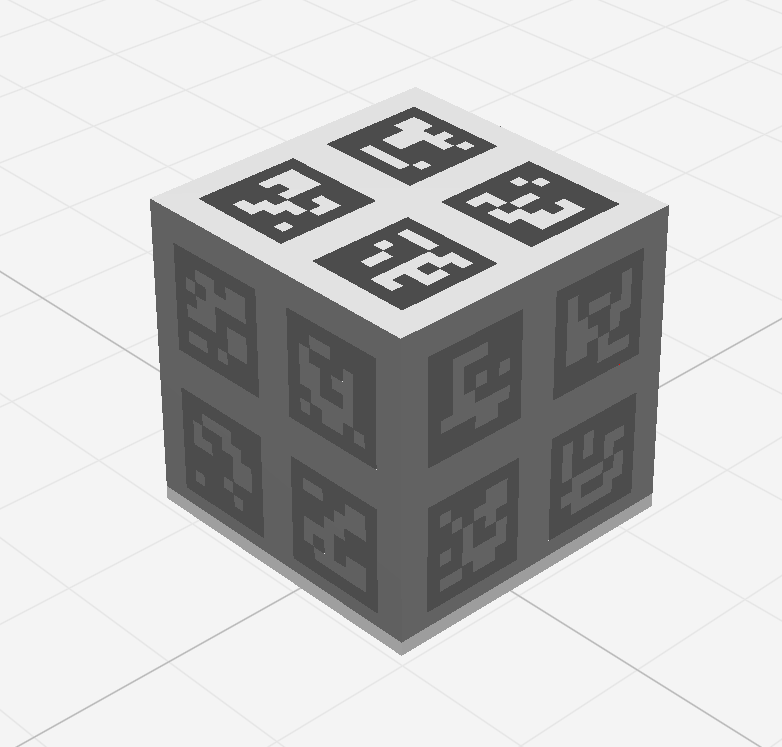
\includegraphics[width=6cm]{imaxes/cubo_marker.png} }}%
    \qquad
    \subfloat[\centering  Impresión del marcador fiduciario.]{{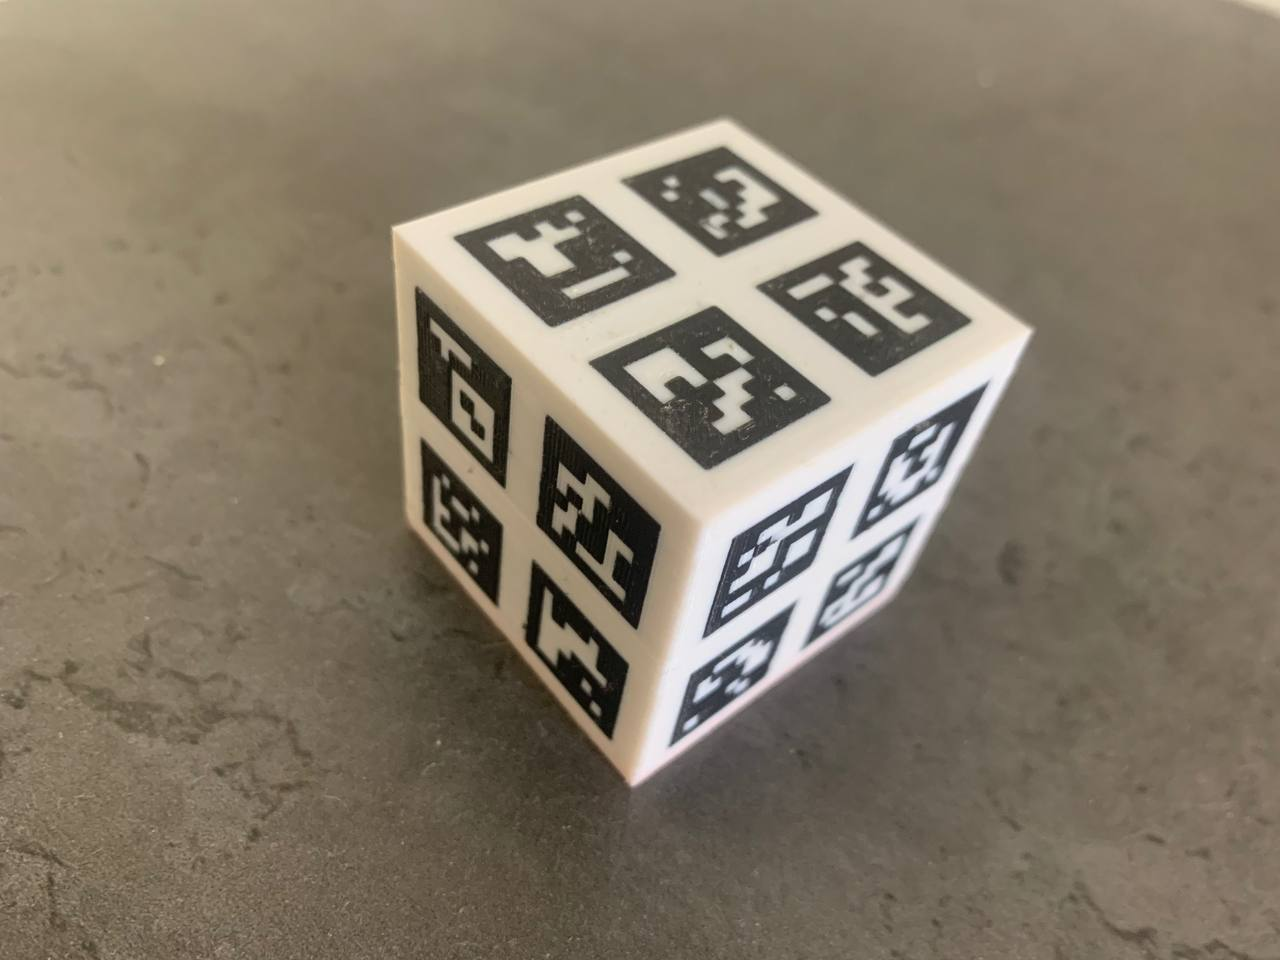
\includegraphics[width=6cm]{imaxes/cubo_marker_imp.png} }}%
    \caption{Diseño final del marcador fiduciario.}%
    \label{fig:3dslier}%
\end{figure}


\section{Implementación del Passthrough en Exposure Render}
Para la obtención de imágenes sobre las que poder trabajar se utilizaron las propias cámaras frontales del HTC Vive Pro 2. Se trata de un par de cámaras colocadas longitudinalmente a lo largo del frontal del casco, que permiten su uso en aplicaciones de realidad aumentada y realidad mixta. 
Para acceder a estas cámaras se debe hacer uso de SRworks C++ SDK. Este software en el momento del desarrollo del trabajo, en su versión nativa, presentaba errores que imposibilitaron la reconstrucción de la imagen para ser visualizada en el casco.
\section{Integración del software de tracking en Exposure Render}
Con el fin de analizar cada imagen con la mínima latencia posible, se implementaron dos threads individuales que esperan cada 16.6ms (ya que las cámaras tienen una tasa de refresco de 60Hz) para obtener una imagen de cada cámara. Dichas imágenes son analizadas para estimar la pose del marcador y modificar la posición del modelo con el que se esta trabajando en Exposure Render.